\chapter{Time Report}

\begin{figure}[H]
  	\centering
  	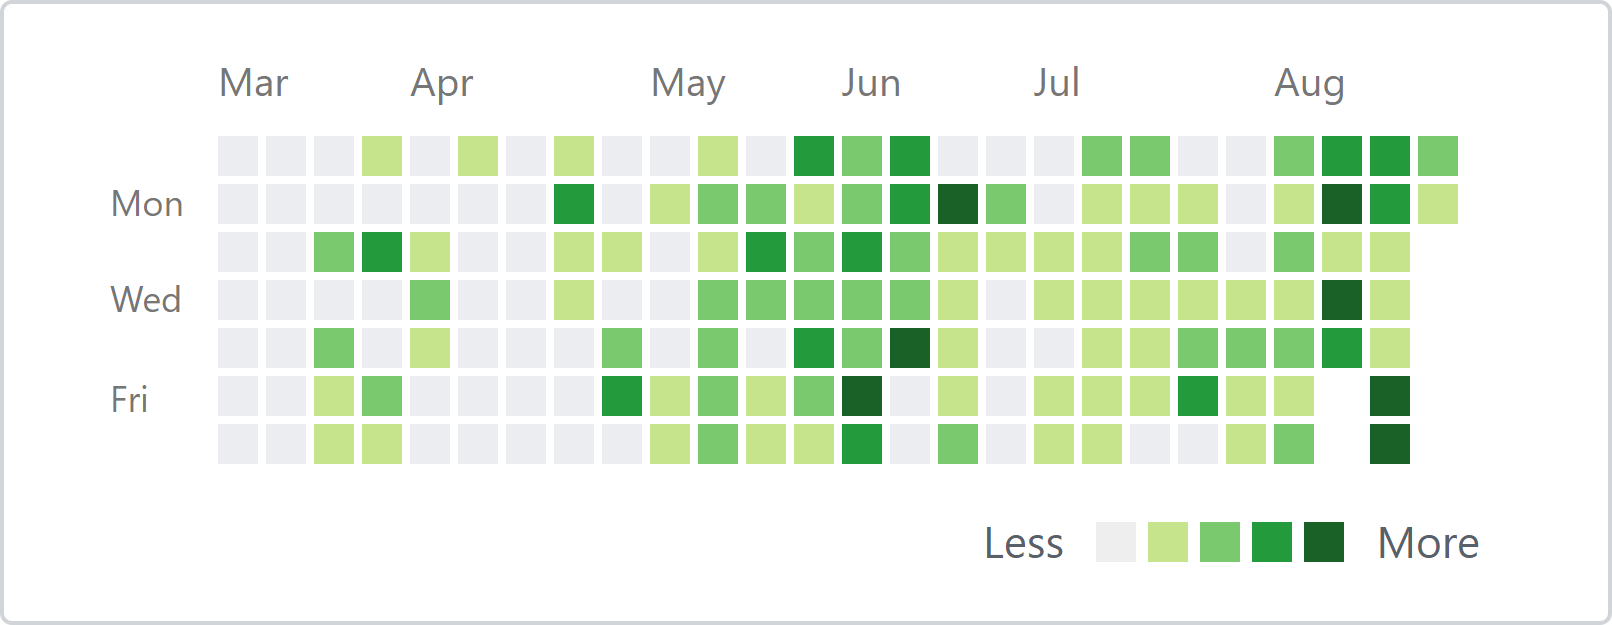
\includegraphics[width=\textwidth]{images/TimeReport}
  	\caption{MicroNet Github commit history.}
  	\label{fig:time_report}
\end{figure}

I did not log any working hours during this semester. In my opinion not writing
hours helps the developer focusing on the actual research tasks instead of
bureaucratic activities. My goal was to only work between six and eight ours per
day to be able to fully concentrate on the work, while ensuring to work at least
six hours. As a compensation for the reduced workload per day I also worked on
most Saturdays and Sundays.

To give an estimation of the actual workload i count six workdays per week with
the minimal six working hours of work per day. I also has two short blocks of
vacation with four respectively six days off. With these assumptions the
estimated working hours of this semester can be calculated.\\

\noindent\textbf{Project duration:} 20. February 2017 - 1. September 2017 = 28
weeks

\noindent\textbf{Total working days:} 28 (weeks) * 6 (days/week) - 10
(vacation) = 158 days

\noindent\textbf{Total working hours:} 158 (days) * 6 (minimal hours/day) = 948
hours\\

\autoref{fig:time_report} shows all activities on the MicroNet repository during
this project. This includes contributions to the framework, the tools, and the
documentation. The two vacation periods are clearly visible in the last week of
June (6 days) and in fourth week of July (4 days). The months at the beginning
of the thesis from February to May show less commits because the literature
research which was conducted in the early stages of the project was
documented with Google Docs.
